\documentclass[a4paper,8pt,twocolumn]{article}
\usepackage[UTF8]{ctex}
\usepackage{graphicx}
\usepackage{fancyhdr}
\usepackage{amsmath}
\usepackage{subcaption}
\usepackage{float}
\usepackage[
  left=2cm, 
  right=2cm,
  top=1.5cm,
  bottom=2.5cm
]{geometry}
\usepackage{pgfplots}
\usepackage{pgfplotstable}
\pgfplotsset{compat=1.18}
\usepackage{siunitx}

\title{
  \textbf{\huge G2 基于 LabVIEW 的虚拟仪器实验报告}}
\author{
  黄雨~24352027\\
\small 中山大学物理学院~广东~广州
}

\begin{document}
\maketitle

\newpage

\section*{实验目的}
\begin{enumerate}
    \item 了解虚拟仪器技术的基本概念。
    \item 学习 LabVIEW 软件开发环境的基本特性及使用方法。
    \item 设计和编制基于 USB 接口的虚拟数据采集器。
    \item 学习 ELVIS II + 虚拟仪器教学平台的使用方法及特性。
\end{enumerate}

\section*{仪器用具}
\begin{itemize}
    \item LabVIEW 软件
    \item NI USB6008 数据采集器
    \item NI ELVIS II + 实验教学平台
    \item 实验测试用计算机 (PC) 及安装了 LabVIEW 软件、NI ELVIS II + 软件、USB6008 驱动程序及相应附件。
\end{itemize}

\section*{实验原理}
\subsection*{1. 数据采集 (DAQ) 的基本原理}
自动化数据采集是将硬件采集到的物理量或数据通过 DAQ 硬件传送到计算机，并通过软件进行处理、分析和显示的过程。本实验将采用台式计算机作为平台，用基于 USB 接口的 USB6008 多功能数据采集模块和 I/O，用 LabVIEW 软件作为虚拟仪器，并用 NI ELVIS II + 教学实验盒作为伴发件。

\subsection*{2. NI ELVIS II + 虚拟仪器教学平台}
利用 NI ELVIS II + 虚拟仪器教学平台作为标准仪器，用于基于 USB6008 数据采集器的虚拟仪器提供标准信号、进行标定。

\subsection*{3. USB6008 多功能数据采集器}
USB6008 是一种多功能数据采集器，它具有 $32$ 个端口，包括 $8$ 个模拟输入 (analog input，AI) 通道、$2$ 个模拟信号输出 (analog output，AO) 通道，以及 $1$ 个 $32$ 位的计数器 (counter)，以及 $12$ 个数字信号输入/输出 (digital input/output，DIO) 端口。
AI 通道在**差分模式** (differential mode) 下使用，可扩展电压测量范围，但该模式下只有 $4$ 个 AI 通道。

\subsection*{4. 安全注意事项}
\begin{itemize}
    \item 利用 NI USB6008 多通道数据采集器的任何一个模拟输入端口的输入电压的峰值不能大于 $\text{10 V}$，而数字信号端口的输入输出电压峰值不能大于 $\text{5.8 V}$，否则会造成损坏。
    \item ELVIS II + 平台的示波器输入信号不能大于 $\text{10 VDC}$、 $\text{7 Vrms}$，数字万用表输入信号不能大于 $\text{60 VDC}$、 $\text{20 Vrms}$，数字信号端口输入输出电压不能大于 $\text{5.8 V}$。使用前请认真阅读说明书。
\end{itemize}

\section*{实验内容与步骤}
\subsection*{（一）学习并掌握 LabVIEW 软件的基本特性和使用方法}
\begin{enumerate}
    \item 打开计算机进入 Windows 操作系统，并启动 LabVIEW 软件。
    \item 根据 LabVIEW 入门指南，完成其中的练习。
\end{enumerate}

\subsection*{（二）了解 ELVIS II + 平台的基本功能}
\begin{enumerate}
    \item 阅读 NI ELVIS II + User Manual，了解 $12$ 种仪器的端口分布及使用方法。
    \item 将 ELVIS II + 平台与计算机以一根 USB 口相连，将变压器输出端插接 ELVIS II + 电源插孔，接通 ELVIS II + 的电源开关。
    \item 运行 “NI ELVISmx Instrument Launcher” 软件，了解并掌握集成的 $12$ 种仪器的使用方法。
\end{enumerate}

\subsection*{（三）利用 LabVIEW 编制 USB6008 各项功能的基本应用方法}
\begin{enumerate}
    \item \textbf{利用 USB6008}
    \begin{enumerate}
        \item 阅读说明书，了解 USB6008 每个端口功能、信号类型和使用方法。
        \item 将 USB6008 与计算机的 USB 口相连。如果 USB6008 上的绿色指示灯闪烁，则说明该设备安装正确，否则需检查连接线。
        \item 检查 USB6008 设备安装是否正常。运行专门用于虚拟仪器管理和检测的 NI MAX (Measurement \& Automation Explorer) 工具。
        \item \textbf{模拟输入 (AI)}：打开测试面板，并设置 AI 信号采集为差分模式， “模式” 选择 “连续”， “输入配置” 选择 “差分”。
        \item 运行 ELVIS II + 的可编程电源 (DPS) 分别输出 DC 电压：$\text{0.5 V}$、 $\text{1 V}$、 $\text{5.0 V}$ 直流信号，并将该信号分别输入 USB6008 的 $\text{AI 0}$ $\sim \text{AI 3}$ 端口。用 LabVIEW 软件编制一个虚拟数字万用表，进行电压测量，记录测量值并作四个端口的输入电压标定曲线。
        \item \textbf{模拟输出 (AO)}：运行 ELVIS II + 的信号发生器 (FGEN) 输出正弦波 ($\text{U}_{\text{P-P}} = \text{2 V}$、 $\text{f} = \text{100 Hz}$)，将信号分别输入 USB6008 的 $\text{AI 0}$ $\sim \text{AI 3}$ 端口。编制一个虚拟示波器，观察并记录测量值。
        \item \textbf{数字 I/O 和计数器 I/O 端口}：在 $\text{ELVIS II +}$ 的数字万用表 ($\text{DMM}$) 测量模式下，选择电压 ($\text{Voltage}$) 在 $\text{0} \sim \text{5 V}$ 档次并按下开关，由接线排 $\text{H9}$ 端口 $\text{14}$ ($\text{P1.4}$) 和 $\text{16}$ ($\text{P1.6}$) 输出电压 ($\text{Output Voltage}$) 在 $\text{0} \sim \text{5 V}$ 之间取若干个电压。并由接线排 $\text{H9}$ 端口 $\text{11}$ ($\text{P1.1}$) 和 $\text{13}$ ($\text{P1.3}$) 输出电压 ($\text{Output Voltage}$) 最小和最大值，最后记录输出电压标定曲线。
    \end{enumerate}
    \item \textbf{编制 LabVIEW 虚拟仪器}
    \begin{enumerate}
        \item 利用 LabVIEW 对 USB6008 进行编程，编制一个虚拟四通道数字电压表，在 USB6008 的 $\text{AI 0}$ $\sim \text{AI 3}$ 端口分别输入 DC 电压：$\text{0.5 V}$、 $\text{1 V}$、 $\text{2 V}$、 $\text{5.0 V}$ 直流，并用虚拟数字电压表测量各端口输入电压的大小，作各端口输入电压标定曲线。
        \item 利用 LabVIEW 对 USB6008 进行编程，编制一个虚拟函数信号发生器，控制 USB6008 的 $\text{AO 0}$ 和 $\text{AO 1}$ 端口分别输出 $\text{0} \sim \text{5 V}$ 直流；$\text{U}_{\text{P-P}} = \text{1 V}$、 $\text{f} = \text{10 Hz}$ 的正弦波；$\text{U}_{\text{P-P}} = \text{1 V}$、 $\text{f} = \text{100 Hz}$ 的方波等三种信号。用示波器观察波形并记录波形。
        \item 利用 LabVIEW 对 USB6008 进行编程，编制一个虚拟简易示波器，并分别在 USB6008 的 $\text{AI 0}$ 端口输入 $\text{1.5 V}$ 直流，在 $\text{AI 1}$ 端口输入 $\text{U}_{\text{P-P}} = \text{1 V}$、 $\text{f} = \text{10 Hz}$ 的正弦波，在 $\text{AI 2}$ 端口输入 $\text{U}_{\text{P-P}} = \text{1 V}$、 $\text{f} = \text{100 Hz}$ 的方波，$\text{AI 3}$ 端口不输入任何信号。用该虚拟示波器同时显示四个通道的信号波形，并解释现象。
    \end{enumerate}
\end{enumerate}

\section*{实验数据记录与结果分析}
\begin{enumerate}
    \item \textbf{AI 端口电压测量与标定记录} (记录输入电压、测量值、标定曲线等)
     \begin{figure}[h]
     \centering
     \begin{tikzpicture}
        \begin{axis}[
            title={\text{AI 端口电压测量与标定记录}},
            xlabel={$U_1/V$},
            ylabel={$U_2/V$},
            xmin=0, xmax=5,
            ymin=0, ymax=5,
            grid=major, % 显示网格
            legend style={at={(0.5,-0.2)},anchor=north} % 图例位置
        ]

        \addplot[
            mark=*,          % 显示标记（实心圆）
            blue,            % 颜色为蓝色
            line width=1pt   % 添加线宽，明确是折线
        ] table {
            % 您的数据 (X Y)
            0   0.201
            0.5 0.507
            1.0 0.995
            1.5 1.496
            2.0 1.996
            2.5 2.496
            3.0 2.992
            3.5 3.485
            4.0 3.987
            4.5 4.484
            5.0 4.977
            
        };
        \addlegendentry{ai 0};
        \addplot[
            mark=*,          % 显示标记（实心圆）
            red,
            line width=1pt   % 添加线宽，明确是折线
        ] table {
            % 您的数据 (X Y)
            0   0.203
            0.5 0.508
            1.0 0.996
            1.5 1.497
            2.0 1.996
            2.5 2.497
            3.0 2.992
            3.5 3.490
            4.0 3.988
            4.5 4.485
            5.0 4.977
            
        };
        \addlegendentry{ai 1};
        \addplot[
            mark=*,          % 显示标记（实心圆）
            green,
            line width=1pt   % 添加线宽，明确是折线
        ] table {
            % 您的数据 (X Y)
            0   0.204
            0.5 0.508
            1.0 0.996
            1.5 1.497
            2.0 1.996
            2.5 2.497
            3.0 2.993
            3.5 3.490
            4.0 3.988
            4.5 4.485
            5.0 4.977
            
        };
        \addlegendentry{ai 2};
        \addplot[
            mark=*,          % 显示标记（实心圆）
            yellow,
            line width=1pt   % 添加线宽，明确是折线
        ] table {
            % 您的数据 (X Y)
            0   0.210
            0.5 0.508
            1.0 0.996
            1.5 1.497
            2.0 1.996
            2.5 2.497
            3.0 2.992
            3.5 3.490
            4.0 3.988
            4.5 4.485
            5.0 4.978
            
        };
        \addlegendentry{ai 3};

        \end{axis}
      \end{tikzpicture}
      \caption{AI 端口电压测量与标定记录}
     \end{figure}

     \begin{figure}[H]
      \centering
       \begin{subfigure}[b]{0.9\linewidth}
        \centering
         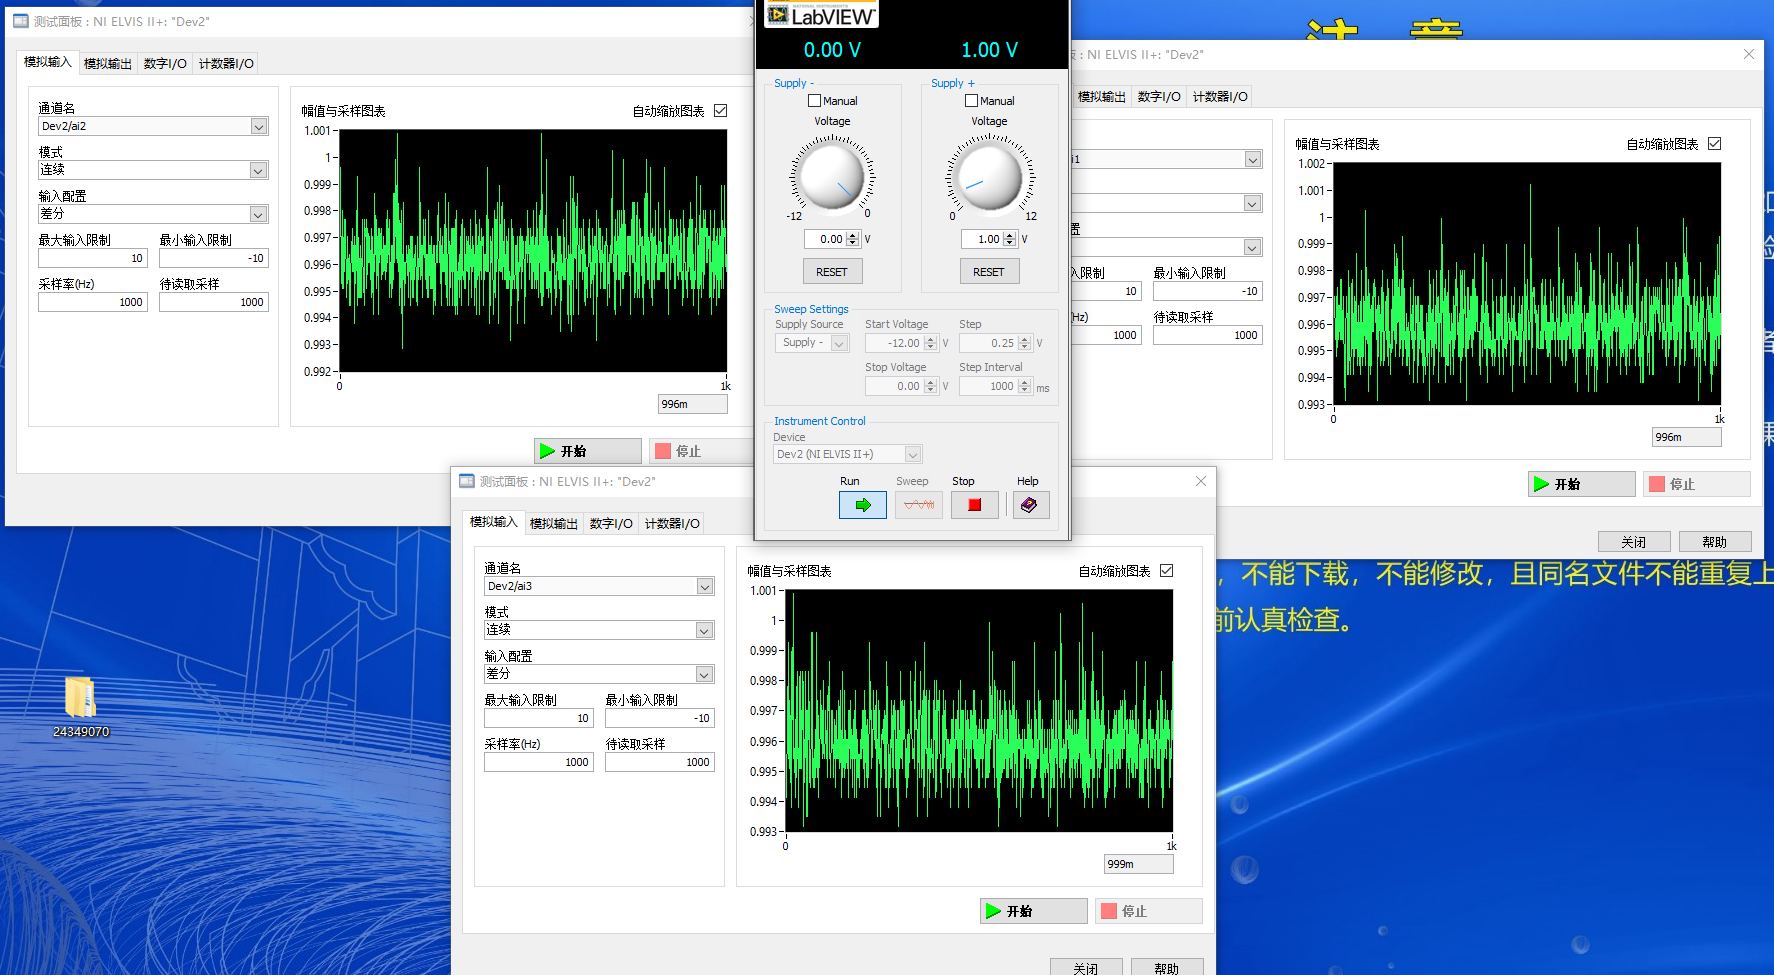
\includegraphics[width=\linewidth]{1.1.png}
        \caption{AI 端口电压 1}
        \label{1.1}
       \end{subfigure}
       \begin{subfigure}[b]{0.9\linewidth}
        \centering
        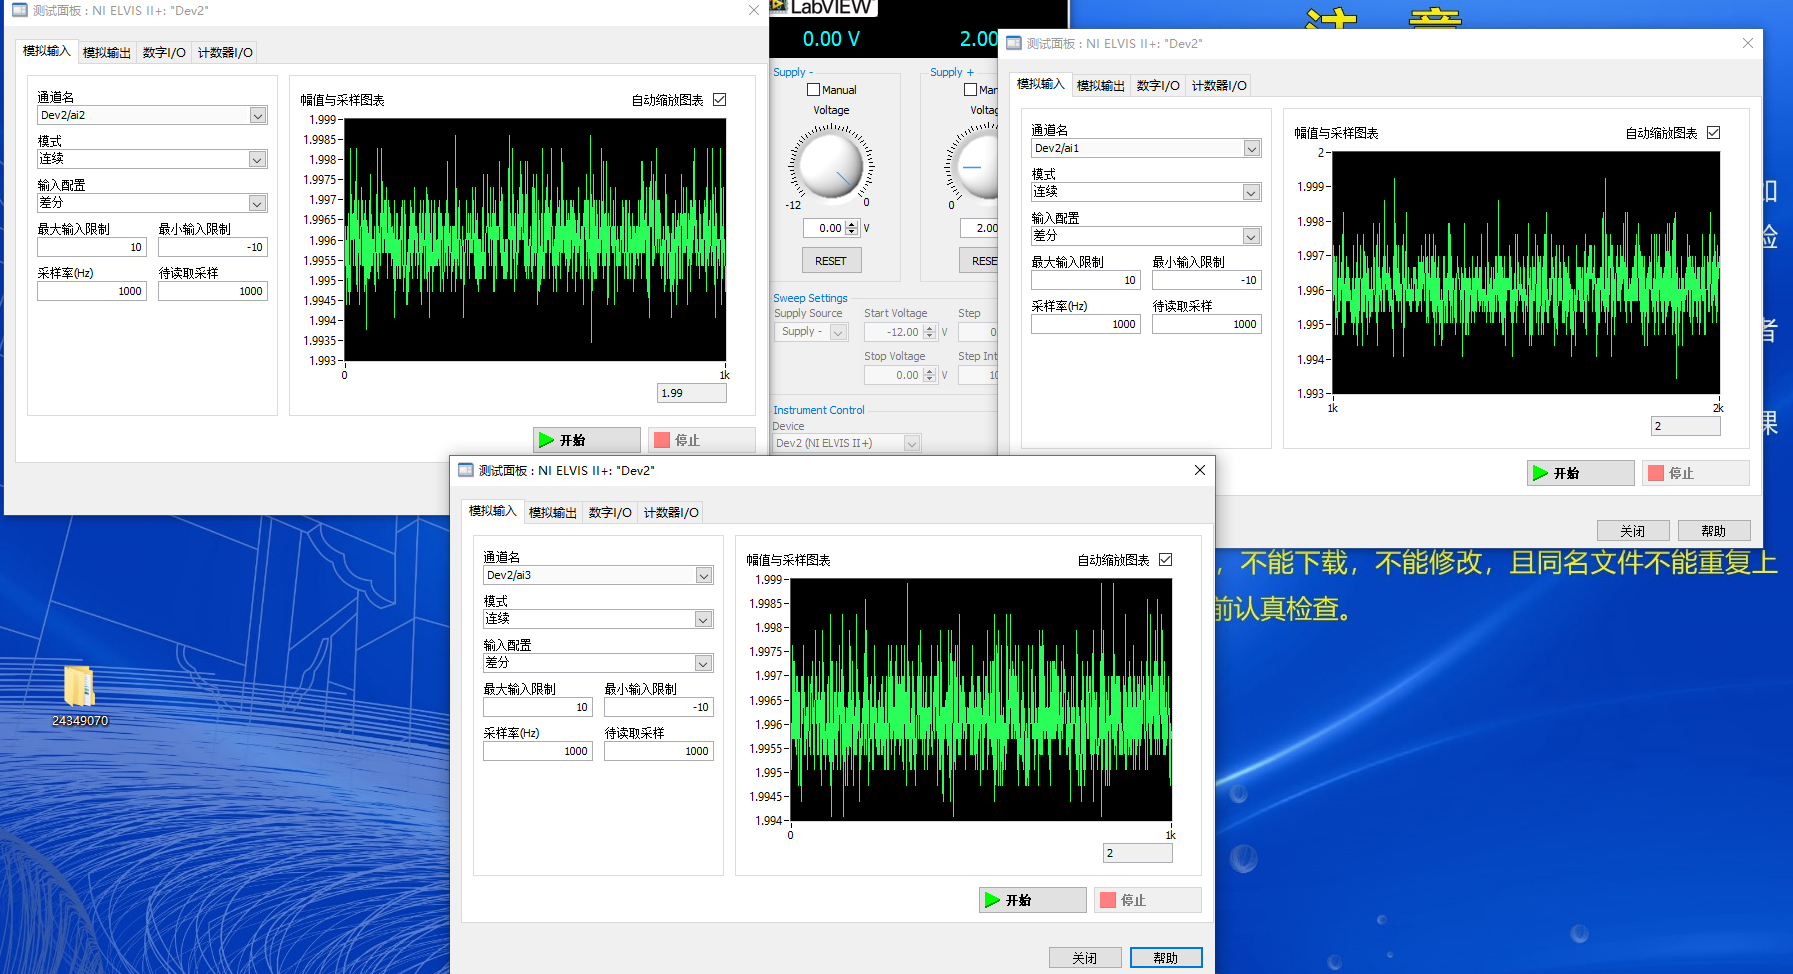
\includegraphics[width=\linewidth]{1.2.png}
        \caption{AI 端口电压 2}
        \label{1.2}
       \end{subfigure}

       \caption{AI 端口电压}
       \label{Figure 1}
      \end{figure}

      \begin{table}[H]
      \centering
       \begin{tabular}{|c|c|}
        \hline
        $\text{端口}$ & $\Delta U/V$\\ 
        \hline
        $ai0$ & $4.0$ \\ 
        \hline
        $ai1$ & $4.0$ \\
        \hline
        $ai2$ & $4.0$ \\
        \hline
        $ai3$ & $4.0$ \\
        \hline
       \end{tabular}
      \caption{AI 端口信号输出正弦信号}
      \label{Date_1}
     \end{table}

     \captionsetup{type=figure}

     \noindent
     \captionof{figure}{AI 输入正弦信号端口面板}
     \label{Figure 2}

     \noindent
     \begin{subfigure}[t]{0.9\linewidth}
      \centering
      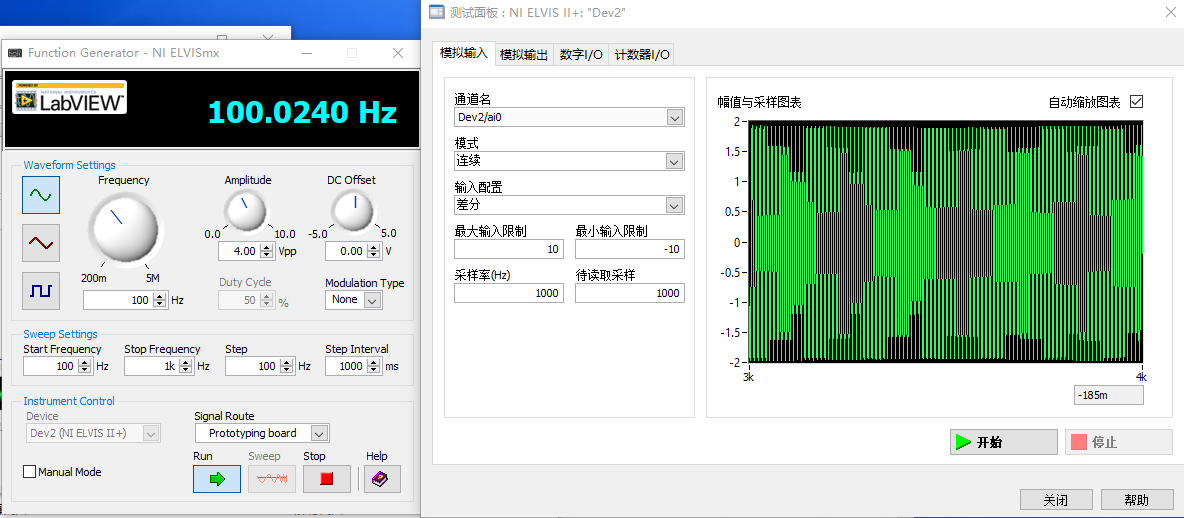
\includegraphics[width=\linewidth]{1.3.png}
      \caption{AI 端口面板 1}
      \label{1.3}
     \end{subfigure}
     \begin{subfigure}[t]{0.9\linewidth}
      \centering
      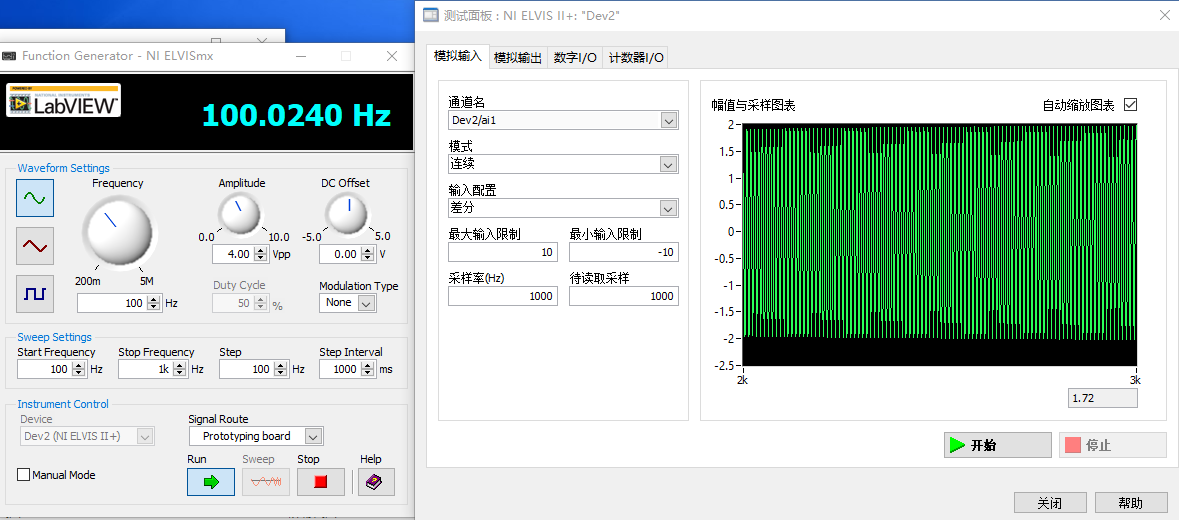
\includegraphics[width=\linewidth]{1.4.png}
      \caption{AI 端口面板 2}
      \label{1.4}
     \end{subfigure}

     \medskip

     \noindent
     \begin{subfigure}[t]{0.9\linewidth}
      \centering
      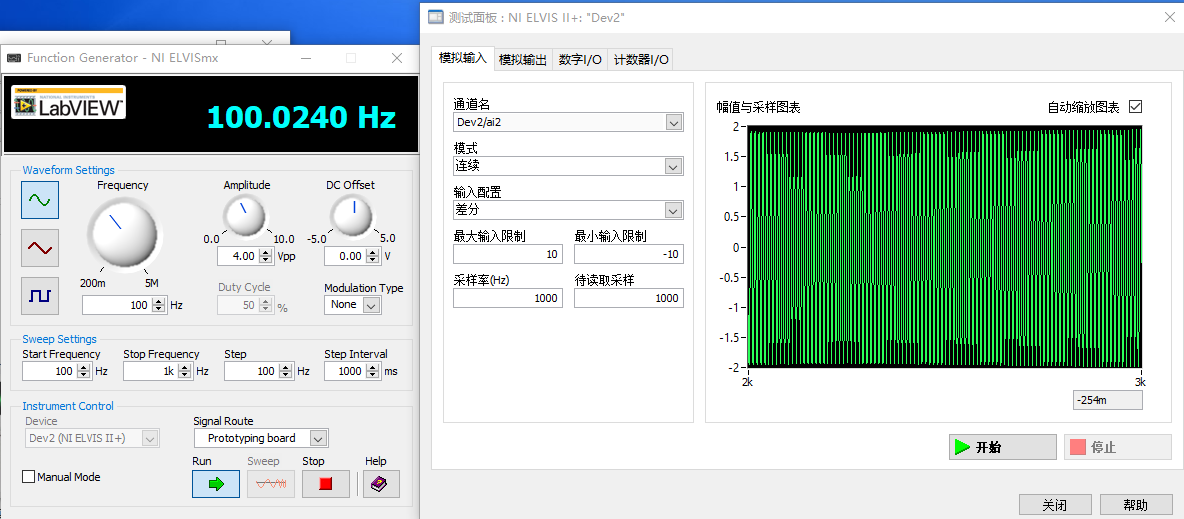
\includegraphics[width=\linewidth]{1.5.png}
      \caption{AI 端口面板 3}
      \label{1.5}
     \end{subfigure}
     \begin{subfigure}[t]{0.9\linewidth}
      \centering
      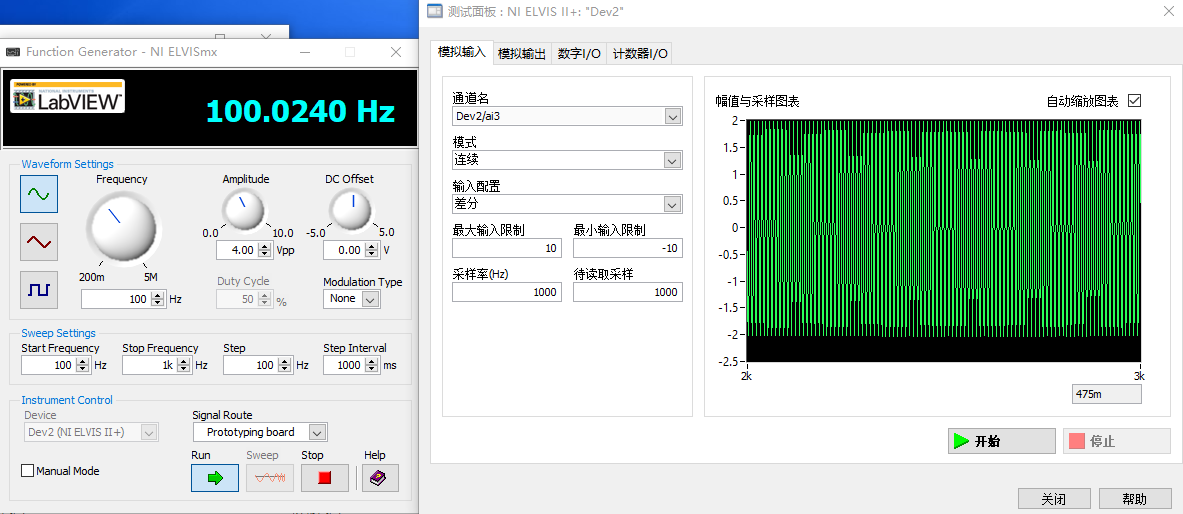
\includegraphics[width=\linewidth]{1.6.png}
      \caption{AI 端口面板 4}
      \label{1.6}
     \end{subfigure}

     
    \item \textbf{AO 端口信号输出波形记录} 
     \begin{figure}[H]
     \centering
     \begin{tikzpicture}
        \begin{axis}[
            title={\text{AO 端口电压测量与标定记录}},
            xlabel={$U_1/V$},
            ylabel={$U_2/V$},
            xmin=0, xmax=5,
            ymin=0, ymax=5,
            grid=major, % 显示网格
            legend style={at={(0.5,-0.2)},anchor=north} % 图例位置
        ]

        \addplot[
            mark=*,          % 显示标记（实心圆）
            blue,            % 颜色为蓝色
            line width=1pt   % 添加线宽，明确是折线
        ] table {
            % 您的数据 (X Y)
            0   0.0510
            0.5 0.4997
            1.0 0.9997
            1.5 1.4994
            2.0 1.9994
            2.5 2.4991
            3.0 2.9991
            3.5 3.4988
            4.0 3.9986
            4.5 4.4986
            5.0 4.9983
            
        };
        \addlegendentry{ao 0};
       
        \end{axis}
      \end{tikzpicture}
      \caption{AO 端口电压测量与标定记录}
     \end{figure}
    \item \textbf{Counter I/O端口的检测}
     \begin{figure}[H]
      \centering
       \begin{subfigure}[b]{0.9\linewidth}
        \centering
         
\includegraphics[width=\linewidth]{3.1.png}
        \caption{输出信号}
        \label{3.1}
       \end{subfigure}
       \begin{subfigure}[b]{0.9\linewidth}
        \centering
        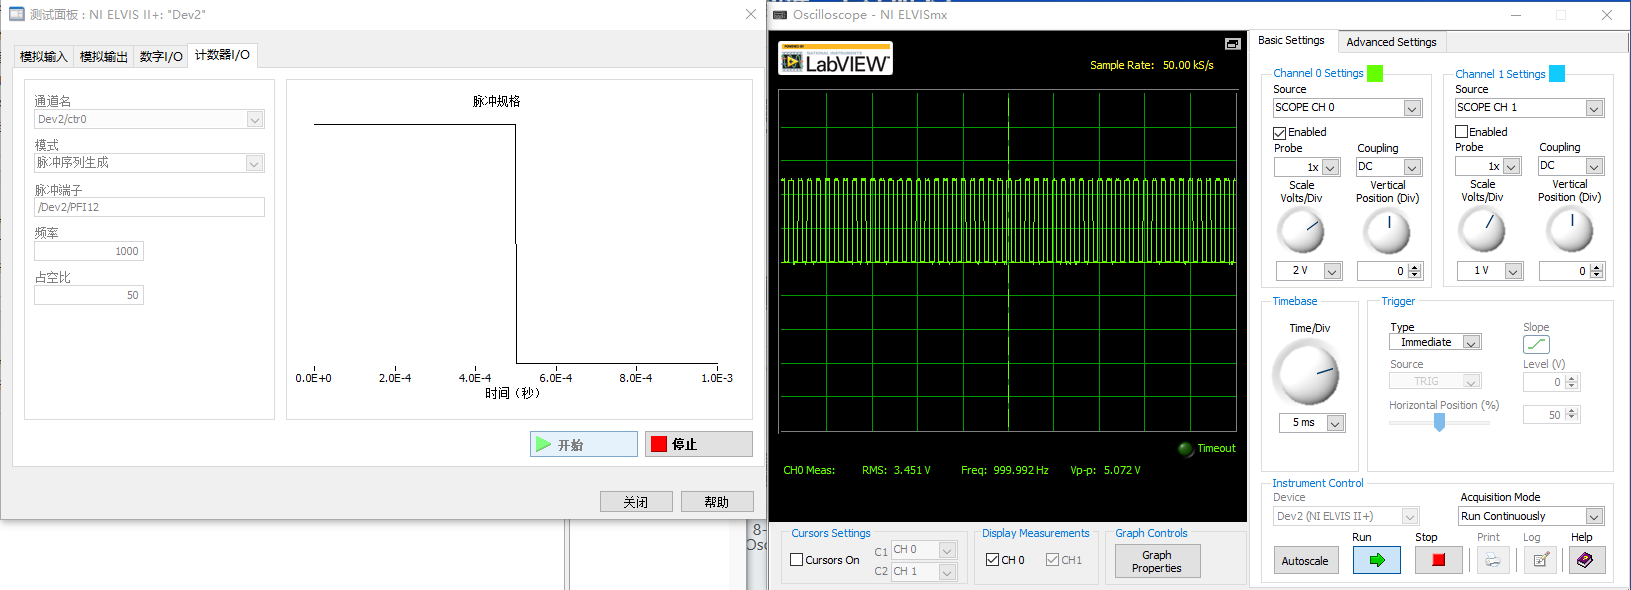
\includegraphics[width=\linewidth]{3.2.png}
        \caption{示波器图像}
        \label{3.2}
       \end{subfigure}

       \caption{Counter I/O端口的检测}
       \label{Figure 3}
      \end{figure}
    \item \textbf{LabVIEW编写虚拟电压表标定AI端口}
     \begin{figure}[h]
     \centering
     \begin{tikzpicture}
        \begin{axis}[
            title={\text{LabVIEW编写虚拟电压表标定AI端口}},
            xlabel={$U_1/V$},
            ylabel={$U_2/V$},
            xmin=0, xmax=5,
            ymin=0, ymax=5,
            grid=major, % 显示网格
            legend style={at={(0.5,-0.2)},anchor=north} % 图例位置
        ]

        \addplot[
            mark=*,          % 显示标记（实心圆）
            blue,            % 颜色为蓝色
            line width=1pt   % 添加线宽，明确是折线
        ] table {
            % 您的数据 (X Y)
            0   0.341
            0.5 0.509
            1.0 0.997
            1.5 1.499
            2.0 1.997
            2.5 2.499
            3.0 2.994
            3.5 3.492
            4.0 3.990
            4.5 4.485
            5.0 4.979
            
        };
        \addlegendentry{ai 0};
        \addplot[
            mark=*,          % 显示标记（实心圆）
            red,
            line width=1pt   % 添加线宽，明确是折线
        ] table {
            % 您的数据 (X Y)
            0   0.302
            0.5 0.473
            1.0 0.960
            1.5 1.458
            2.0 1.958
            2.5 2.459
            3.0 2.950
            3.5 3.447
            4.0 3.944
            4.5 4.439
            5.0 4.933
            
        };
        \addlegendentry{ai 1};
        \addplot[
            mark=*,          % 显示标记（实心圆）
            green,
            line width=1pt   % 添加线宽，明确是折线
        ] table {
            % 您的数据 (X Y)
            0   0.341
            0.5 0.510
            1.0 0.997
            1.5 1.499
            2.0 1.998
            2.5 2.499
            3.0 2.994
            3.5 3.491
            4.0 3.990
            4.5 4.486
            5.0 4.978
            
        };
        \addlegendentry{ai 2};
        \addplot[
            mark=*,          % 显示标记（实心圆）
            yellow,
            line width=1pt   % 添加线宽，明确是折线
        ] table {
            % 您的数据 (X Y)
            0   0.341
            0.5 0.510
            1.0 0.999
            1.5 1.499
            2.0 1.999
            2.5 2.499
            3.0 2.994
            3.5 3.492
            4.0 3.990
            4.5 4.487
            5.0 4.979
            
        };
        \addlegendentry{ai 3};

        \end{axis}
      \end{tikzpicture}
      \caption{LabVIEW编写虚拟电压表标定AI端口}
     \end{figure}

     \captionsetup{type=figure}

     \noindent
     \captionof{figure}{AI 端口面板}
     \label{Figure 4}

     \noindent
     \begin{subfigure}[t]{1\linewidth}
      \centering
      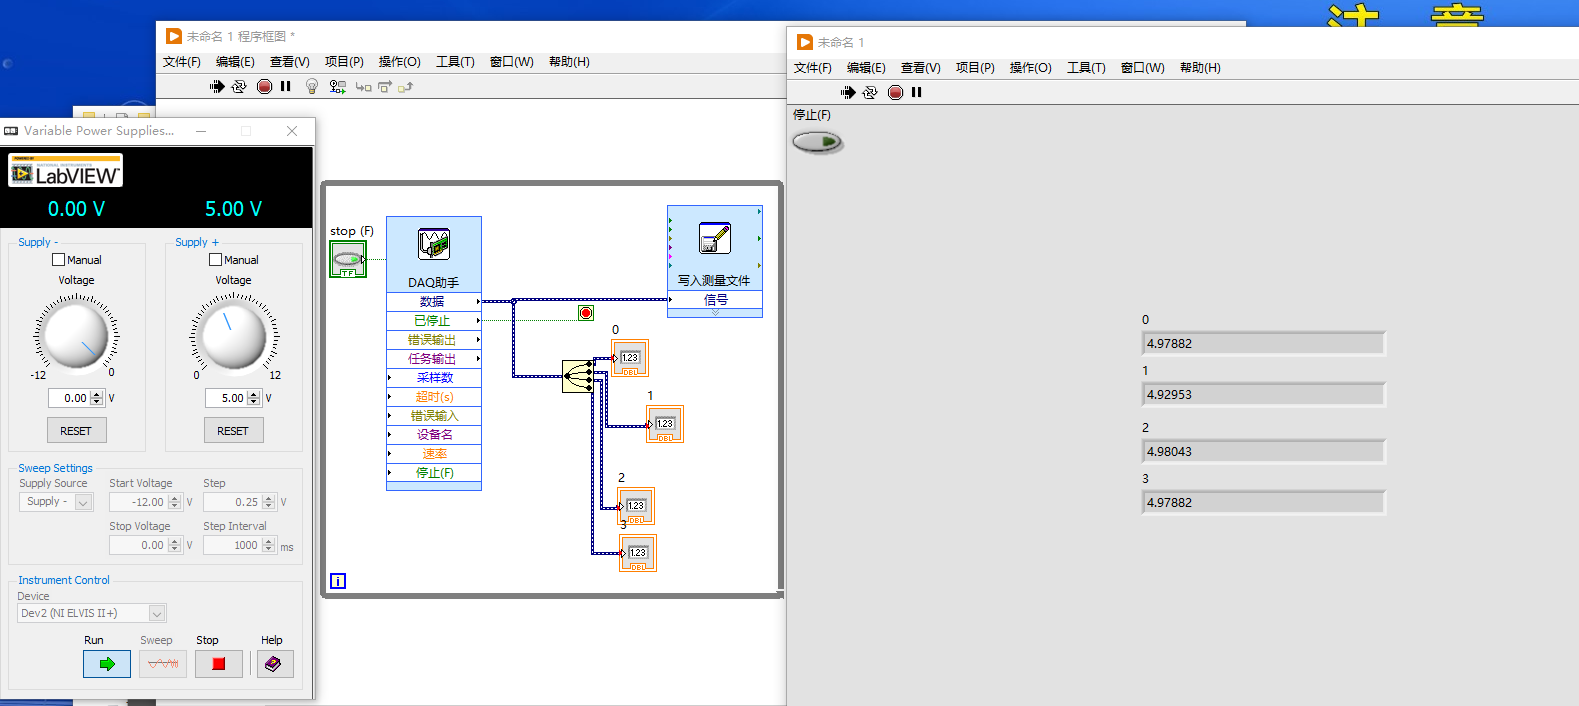
\includegraphics[width=\linewidth]{4.1.png}
      \caption{AI 端口面板 1}
      \label{4.1}
     \end{subfigure}
     \begin{subfigure}[t]{1\linewidth}
      \centering
      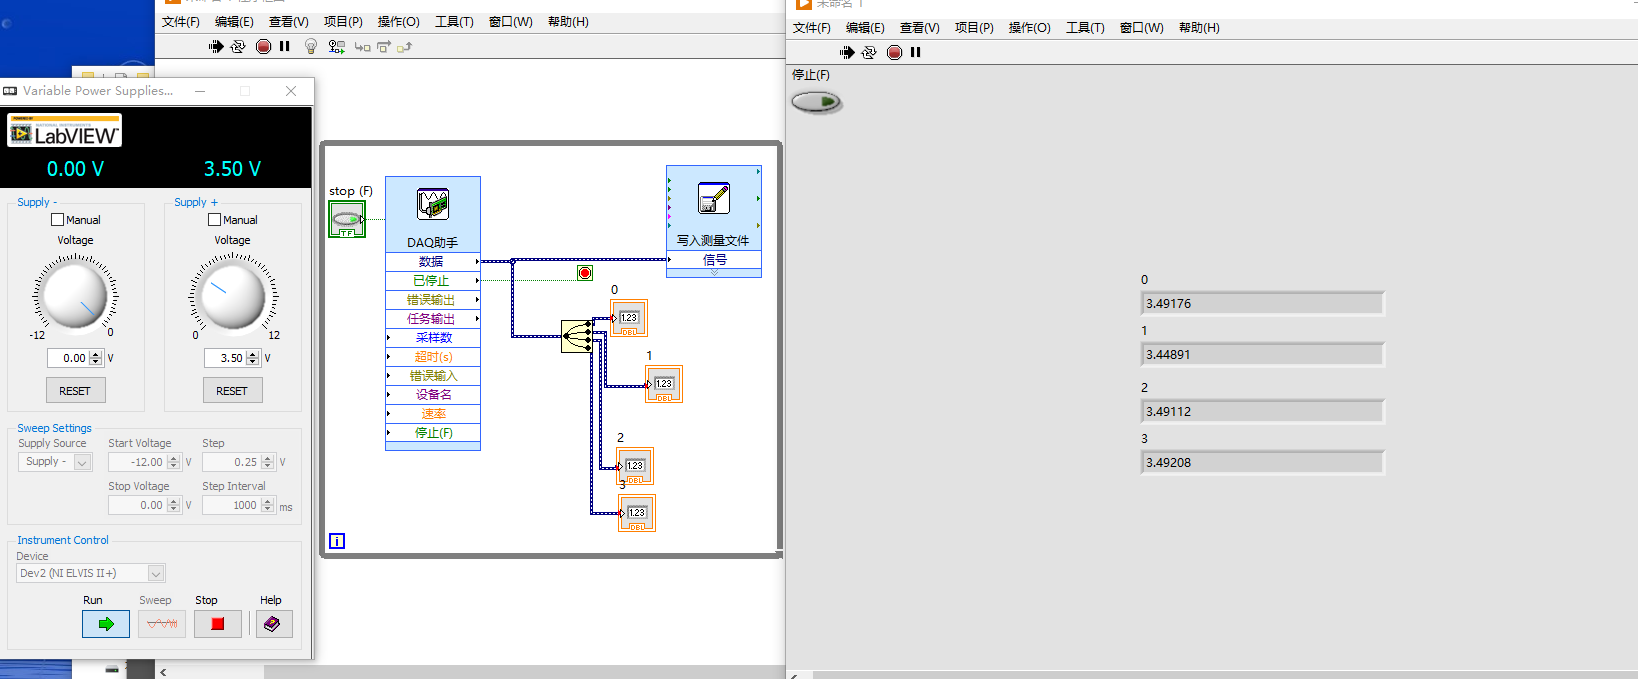
\includegraphics[width=\linewidth]{4.2.png}
      \caption{AI 端口面板 2}
      \label{4.2}
     \end{subfigure}

    \item \textbf{虚拟简易示波器波形显示}
     \captionsetup{type=figure}

     \noindent
     \captionof{figure}{虚拟简易示波器波形显示}
     \label{Figure 5}

     \noindent
     \begin{subfigure}[t]{1\linewidth}
      \centering
      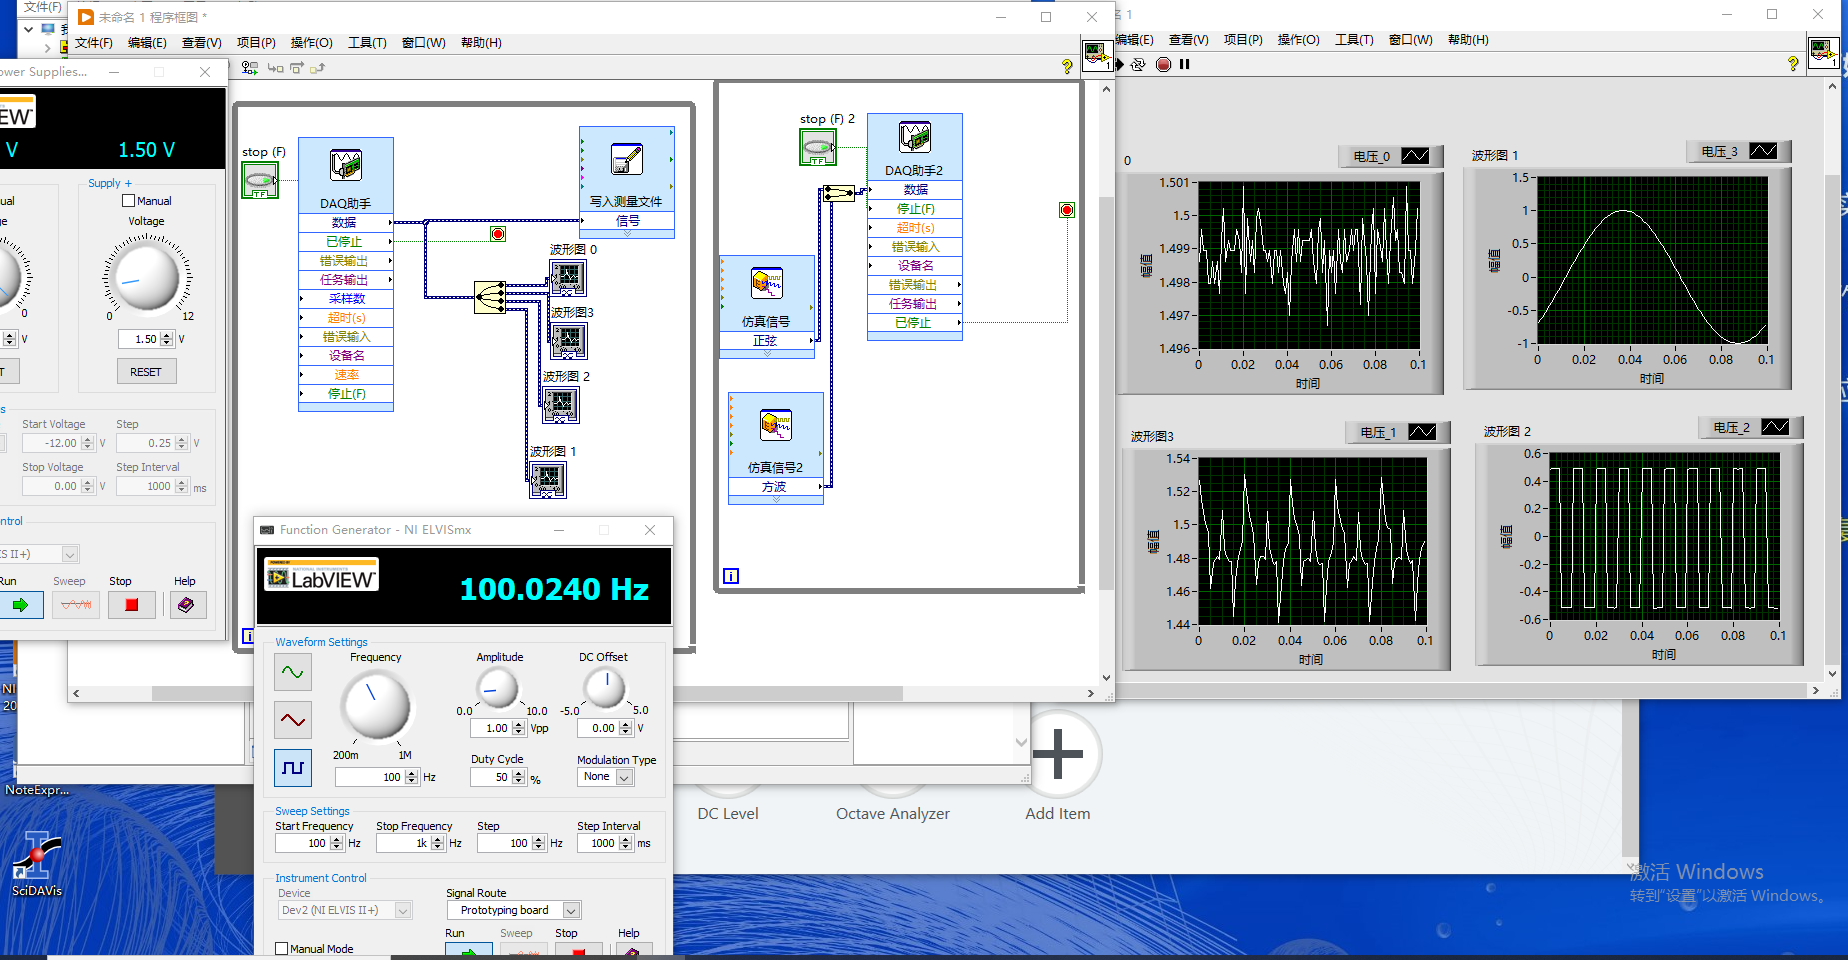
\includegraphics[width=\linewidth]{5.1.png}
      \caption{总面板}
      \label{5.1}
     \end{subfigure}
     \begin{subfigure}[t]{1\linewidth}
      \centering
      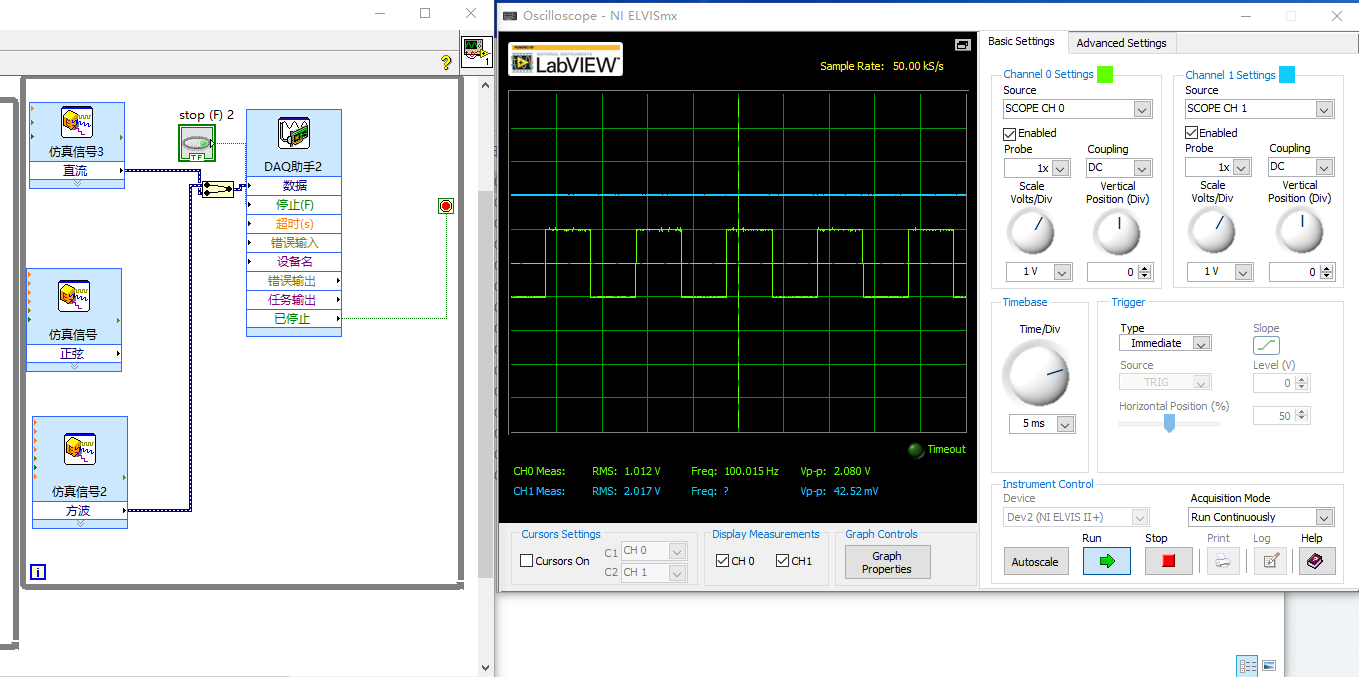
\includegraphics[width=\linewidth]{5.2.png}
      \caption{方波与直流}
      \label{5.2}
     \end{subfigure}
     \begin{subfigure}[t]{1\linewidth}
      \centering
      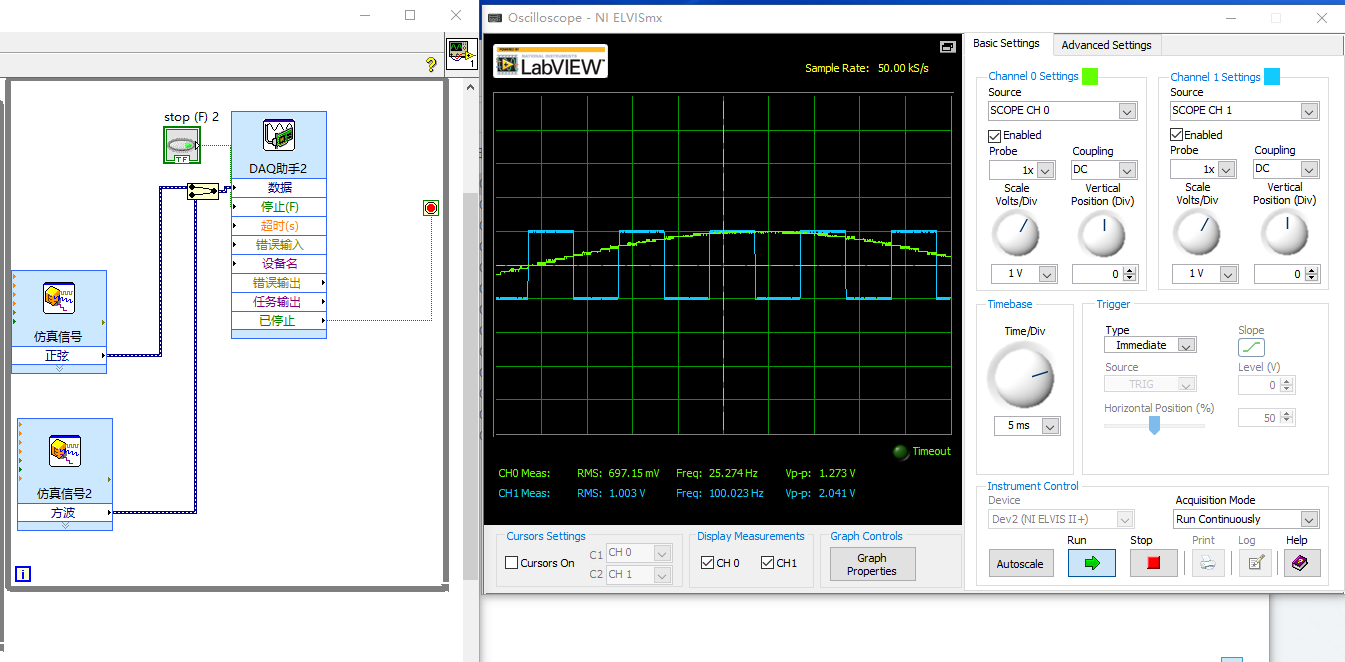
\includegraphics[width=\linewidth]{5.3.png}
      \caption{方波与正弦波}
      \label{5.3}
     \end{subfigure}
     \begin{subfigure}[t]{1\linewidth}
      \centering
      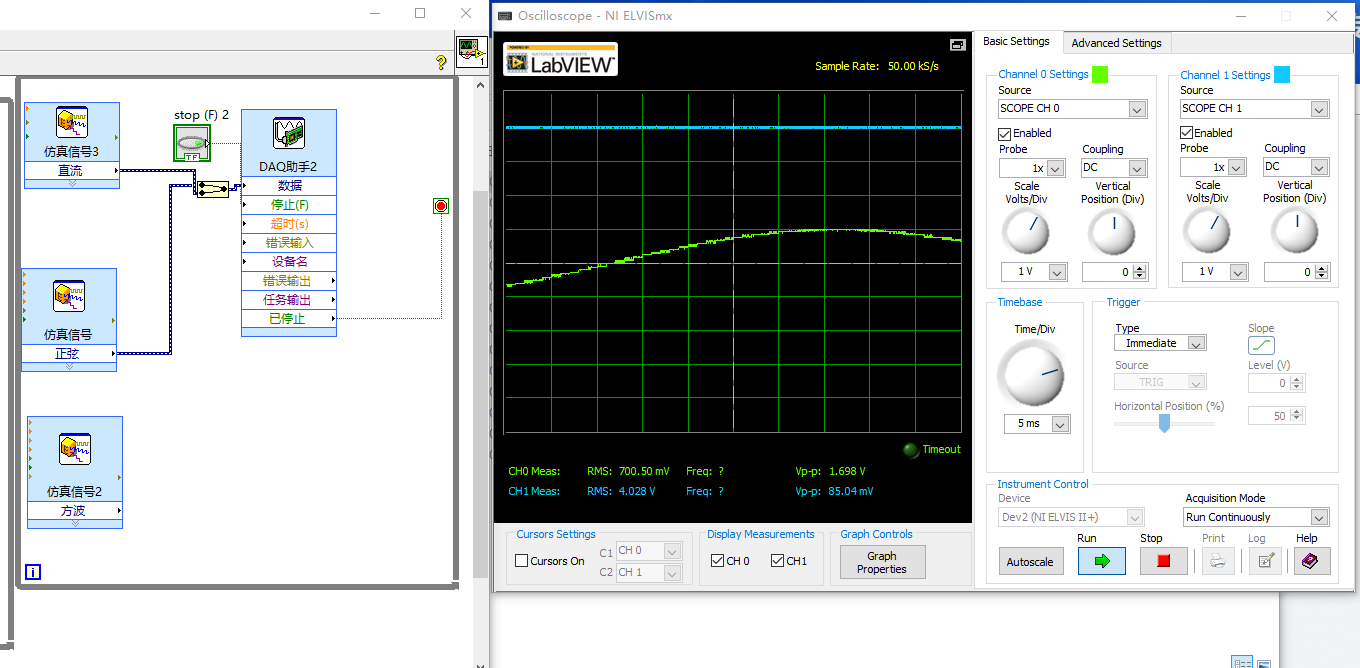
\includegraphics[width=\linewidth]{5.4.png}
      \caption{正弦波与直流}
      \label{5.4}
     \end{subfigure}
    \item \textbf{部分电路连接展示}
     \captionsetup{type=figure}

     \noindent
     \captionof{figure}{部分电路连接展示}
     \label{Figure 5}

     \noindent
     \begin{subfigure}[t]{1\linewidth}
      \centering
      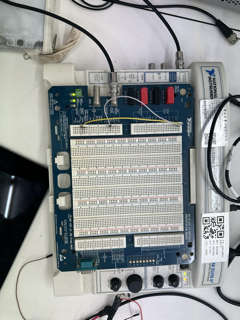
\includegraphics[width=\linewidth]{6.1.png}
      \caption{实验电路 1}
      \label{6.1}
     \end{subfigure}
     \begin{subfigure}[t]{1\linewidth}
      \centering
      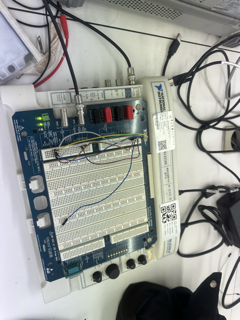
\includegraphics[width=\linewidth]{6.2.png}
      \caption{实验电路 2}
      \label{6.2}
     \end{subfigure}
     \begin{subfigure}[t]{1\linewidth}
      \centering
      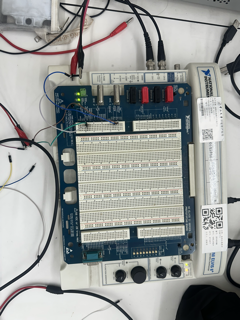
\includegraphics[width=\linewidth]{6.3.png}
      \caption{实验电路 3}
      \label{6.3}
     \end{subfigure}
\end{enumerate}


\section*{思考题}
\begin{enumerate}
  \item \textbf{虚拟仪器与传统的测量仪器相比有什么异同？虚拟仪器能否用来进行测量？}

  虚拟仪器与传统仪器的区别在于：传统仪器由硬件固定功能实现测量；虚拟仪器由通用硬件（如数据采集卡）与软件（如 LabVIEW）结合，通过编程实现多种测量功能。虚拟仪器可以进行实际测量。

  \item \textbf{一台能正常工作的虚拟仪器包括几项必要组成部分？}

  一台正常工作的虚拟仪器包括：
  \begin{itemize}
    \item 数据采集硬件（如 NI USB6008）；
    \item 信号调理电路；
    \item 计算机；
    \item 测量与控制软件（如 LabVIEW 程序）。
  \end{itemize}

  \item \textbf{试述利用 NI USB6008 多功能数据采集器和 LabVIEW 软件制作一个虚拟数字万用表。}

  使用 NI USB6008 和 LabVIEW 可制作虚拟数字万用表。软件中实现信号采集、处理与显示模块，可测量电压、电流、电阻、频率等参数。

  \item \textbf{试编制一个多通道的数据采集器。}

  采样时间间隔可在 1 s～10 min 内调节；采集到的数据应包括数据编号、采样时间、测量电压等信息，并同步保存至用户指定的磁盘文件中。
\end{enumerate}

\clearpage
\onecolumn
\section*{教师签名页}
 \begin{figure}[ht] 
    \centering
    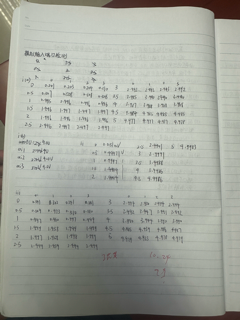
\includegraphics[width=1\textwidth]
    {7.1.png} 
    \caption{教师签名页}
    \label{7.1} 
  \end{figure}

\end{document}